\documentclass[%
    %draft,
    %submission,
    %compressed,
    final,
    %
    %technote,
    %internal,
    %submitted,
    %inpress,
    %reprint,
    %
    %titlepage,
    notitlepage,
    %anonymous,
    narroweqnarray,
    inline,
    twoside,
    invited
    ]{lib/ieee}

\usepackage[utf8]{inputenc}
\usepackage[spanish]{babel}
\usepackage{graphicx}
\usepackage{verbatim}
\usepackage{moreverb}
\usepackage{amsmath}
\usepackage{amsfonts}
\usepackage{amssymb}
\usepackage{fancybox}
\usepackage{float}
\usepackage{fancyvrb}
\usepackage{subfigure}
\usepackage{listings}

\newcommand{\latexiie}{\LaTeX2{\Large$_\varepsilon$}}

%\usepackage{ieeetsp}    % if you want the "trans. sig. pro." style
%\usepackage{ieeetc}    % if you want the "trans. comp." style
%\usepackage{ieeeimtc}    % if you want the IMTC conference style

% Use the `endfloat' package to move figures and tables to the end
% of the paper. Useful for `submission' mode.
%\usepackage {endfloat}

% Use the `times' package to use Helvetica and Times-Roman fonts
% instead of the standard Computer Modern fonts. Useful for the
% IEEE Computer Society transactions.
%\usepackage{times}
% (Note: If you have the commercial package `mathtime,' (from
% y&y (http://www.yandy.com), it is much better, but the `times'
% package works too). So, if you have it...
%\usepackage {mathtime}

% for any plug-in code... insert it here. For example, the CDC style...
%\usepackage{ieeecdc}

\begin{document}

%----------------------------------------------------------------------
% Title Information, Abstract and Keywords
%----------------------------------------------------------------------
\title[PageRank]{%
       PageRank}

% format author this way for journal articles.
% MAKE SURE THERE ARE NO SPACES BEFORE A \member OR \authorinfo
% COMMAND (this also means `don't break the line before these
% commands).
\author[Sneidermanis, Sturla]{Darío Sneidermanis, Martín Sturla\\
\\\textbf{19 de Abril de 2012}
}



\titletext{Métodos\ Numéricos\ Avanzados,\ ITBA\ -\ 19\ de\ abril\ de\ 2012}
\lognumber{}
\pubitemident{}
\loginfo{19 de Abril, 2012.}
\firstpage{1}

\confplacedate{Buenos Aires, Argentina, 19 de Abril, 2012}

\maketitle

\begin{abstract}
Se analizan y compara el desempeño de la implementación clásica del algoritmo de PageRank, con el método de las potencias, y una implementación
alternativa que se empezó a estudiar recientemente, usando sistemas lineales.
\end{abstract}

\begin{keywords}
PageRank, motores de búsqueda, cadenas de Markov, método de las potencias, autovectores.
\end{keywords}

%----------------------------------------------------------------------
% SECTION I: Introduccion%----------------------------------------------------------------------
\section{Introducción}
Con el inicio de las telecomunicaciones masivas por Internet a principio de los 90' y su rápido crecimiento, nació la necesidad de
crear un índice de los sitios web. Estos índices eran usados por los motores de búsqueda, y acompañaron el crecimiento del tráfico
de Internet. En 1994, World Wide Web Worm poseía un índice de unos 110.000 sitios, y era consultado unas 1500 veces diariamente. Ya en
1997, los motores de búsqueda contaban con índices con una cantidad de sitios que variaba desde 2 hasta 100 millones, y algunos eran consultados
unas 20 millones de veces diariamente. Estos índices eran mantenidos por humanos y por lo tanto, además de ser posiblemente subjetivos,
no parecían ser lo suficientemente escalables como para poder acompañar el rápido crecimiento del tráfico por Internet. \\

En 1998, habiendo previsto índices en el orden
de los miles de millones de sitios para el fin del milenio, dos estudiantes de Stanford, Sergey Brin y Lawrance Page, publicaron un paper titulado
\textit{"The Anatomy of a Large-Scale Hypertextual Web Search Engine"} que explora el problema mencionado anteriormente y ofrece una solución; un
algoritmo computable para indexar sitios web según su importancia, conocido como \textit{PageRank}. Estos estudiantes crearon el conocido motor de
búsqueda llamado \textit{Google} utilizando este algoritmo. \\

Se comienza el paper con una exposición y modelado del problema en la sección II, seguido del desarrollo matemático básico en la sección III.
En la sección IV se exponen los dos métodos de solución y se comparan experimentalmente en la sección V.

%----------------------------------------------------------------------
% SECTION II: Que es PageRank?
%----------------------------------------------------------------------

\section{Modelado del problema}

\par El conjunto de los sitios web puede ser representado como un digrafo, donde cada sitio es un nodo. Existe una arista dirigida entre dos nodos si
desde el primer sitio hay un hipervínculo al segundo. El \textit{PageRank} de cada sitio (nodo) es la probabilidad de que una persona apretando hipervínculos al azar
llegue a ese sitio (nodo).
En cada momento o iteración, dicha persona esta en un sitio y puede desplazarse a otro sitio por un hipervínculo al azar (con probabilidad $d$,
llamado factor de amortiguamiento), o ingresar a un sitio al azar de toda la web (usar la barra de direcciones del navegador).

\begin{figure}[h!]
    \centering
    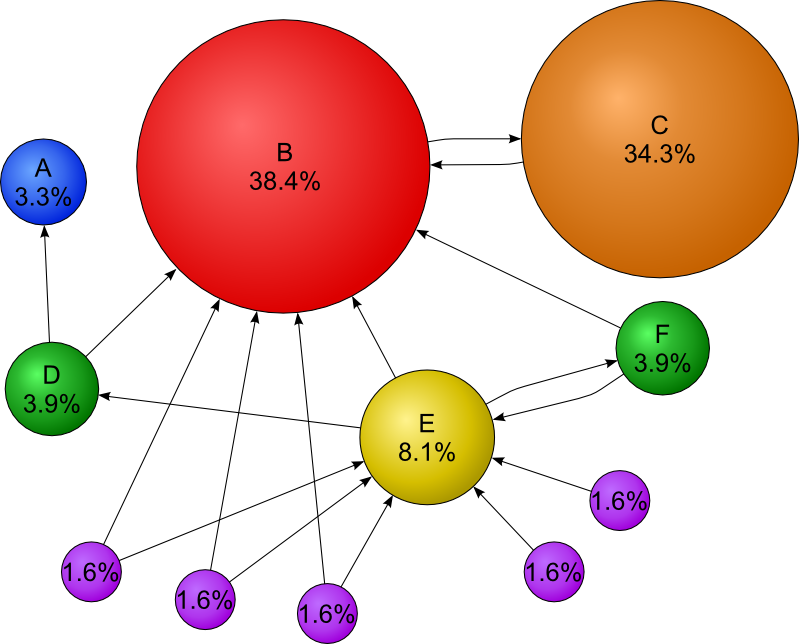
\includegraphics[width=0.5\textwidth]{img/pagerank.png} % [scale=0.75]
    \caption{PageRanks, representados como porcentajes, de una red simple. Nótese que el sitio C tiene un PageRank alto, a pesar de tener solo una arista
             entrante, por ser esta de un sitio importante.}
\end{figure}
%%

En vista de dichas propiedades, este grafo puede ser visto como una cadena de Markov: se toman las probabilidades iniciales de
estar en cualquier nodo uniformemente, y las probabilidades de abrir un hipervínculo de un mismo nodo también uniformemente. Además no existen
estados absorbentes; se asume que en cualquier momento un usuario podría ingresar (con probabilidad $1-d$) el nombre de cualquier otro sitio en el navegador, con distribución
uniforme, nuevamente.\\

El vector de probabilidades al que converge dicha cadena de Markov, representa el peso o importancia de cada sitio: el PageRank, que es una distribucción de probabilidades.
Por lo tanto, el vector debe estar normalizado.

\section{Marco algebraico}

\par Se debe calcular $PR(p_i)$, el valor del \textit{PageRank} de un nodo $p_i$. Dicho valor se calcula como la suma de la probabilidad de haber
llegado por la barra de direcciones (con probabilidad $(1-d)/N$), y haber venido por un hipervínculo de un sitio o nodo $p$: \\

\begin{equation}\label{pranknode}
    PR(p_i) = \frac{1-d}{N} + d \sum_{p \in M_{p_{i}}} \frac{PR(p)}{L(p)}
\end{equation}

Donde $L(p)$ es el grado de salida del nodo $p$, $N$ es la cantidad total de nodos, y $M_{p_i}$ es el conjunto de los nodos que alcanzan directamente a $p_i$.\\

Nota: La probabilidad de haber llegado a través de un hipervínculo, es decir el factor de amortiguamiento $d$, vale aproximadamente $0,85$ (establecido empíricamente [1]).

Aplicando la ecuación \eqref{pranknode} a todos los nodos, se obtiene una nueva ecuación en forma matricial:

\begin{equation}\label{pranksolution}
    R = \begin{pmatrix}
            (1-d)/N \\ (1-d)/N \\ \vdots \\ (1-d)/N
        \end{pmatrix}
        + dMR
\end{equation}

Donde $R$ es el vector de \textit{PageRanks} y $M_{i,j}$ se define como $L(p_j)^{-1}$ si existe un hipervínculo en $p_j$ hacia $p_i$, y $0$ sino.

\[
    R_i = \frac{1-d}{N} + d \sum_{j=1}^{N} M_{i,j} R_j
\]

\section{Soluciones para el problema de calcular el PageRank}

Se define la matriz $\widehat{M}$ como:

\begin{equation}\label{mhat}
    \widehat{M} = \frac{1-d}{N}E + dM
\end{equation}

Donde $E$ es una matriz con todos unos.\\

Usando la ecuación \eqref{pranksolution}:

\begin{eqnarray}
    R &=& \begin{pmatrix}
              (1-d)/N \\ (1-d)/N \\ \vdots \\ (1-d)/N
          \end{pmatrix}
          + dMR \nonumber\\
      &=& \frac{1-d}{N}ER + dMR \nonumber\\
      &=& \widehat{M}R \label{eigenr}
\end{eqnarray}

($E_i \cdot R = 1$, pues $R$ es una distribución de probabilidades)\\

La cadena de Markov con matriz de transición $\widehat{M}$ es ergódica y regular (ya que todas las transiciones son no nulas) y, por lo tanto, R existe y es único (teorema ergódico).

\subsection{Método de las potencias}

Dado que las filas y columnas de
$\widehat{M}$ suman $1$ (es estocástica), por círculos de Gershgorin el módulo de todos los autovalores deberá ser menor o igual a $1$.
De la ecuación \eqref{eigenr} se puede deducir que la solución $R$ no es más que el autovector dominante con autovalor $1$ de la matriz $\widehat{M}$.
El autovalor será único si existe una única distribución que satisface la ecuación \eqref{eigenr}, lo cual es equivalente a exigir
que $Rg\left(\widehat{M}-I\right) = N-1$ y no menor.
Si se cumple, se puede calcular $R$ con el método de las potencias. Cabe destacar que como
$R$ es una distribución de probabilidades, el autovector debe estar normalizado.\\

El método de las potencias consiste en tomar un vector $v(0)$ e iterar según la regla:

\begin{equation}
    v(t+1) = \widehat{M}v(t)
\end{equation}

Normalizando $v(t+1)$ en cada paso, hasta que se cumpla:

\begin{equation}
    \left| v(t+1) - v(t) \right| < \epsilon
\end{equation}

Donde $\epsilon$ es un error adecuado. El método de las potencias converge al autovalor dominante siempre y cuando la proyección del
vector $v(0)$ a este último no sea nula.\\

El ritmo asintótico de convergencia de este método está gobernado por el autovalor subdominante. Este autovalor está acotado
superiormente por $d$, el factor de amortiguamiento [4]. En la figura 1, se puede ver que para $0.5 \leq d \leq 0.9$, el
factor de amortiguamiento afecta linealmente el tiempo de ejecución del algoritmo.
Esto trae a la mesa el interesante trade-off de tiempo de ejecución versus factor de amortiguamiento $d$, que es un dato empírico. Habría que
 analizar cuánto cambia la solución al variar $d$.

\begin{figure}[h!]
    \centering
    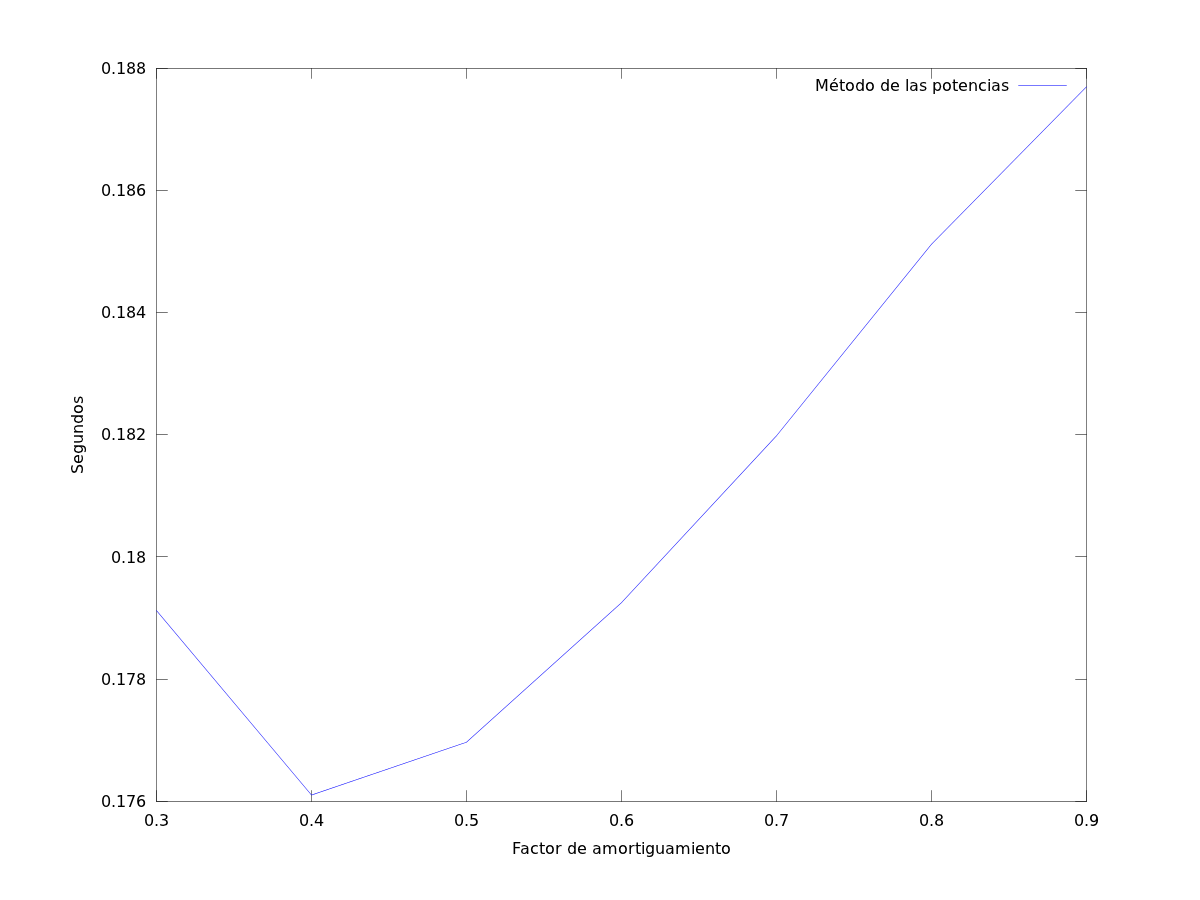
\includegraphics[width=0.5\textwidth]{img/d_pm.png} % [scale=0.75]
    \caption{Gráfico del tiempo de ejecución del método de las potencias en función de el factor de amortiguamiento, para un grafo de 100 sitios.}
\end{figure}

\subsection{Sistema lineal}

De \eqref{pranksolution} se deduce:

\begin{equation}
    (I - dM) R = \begin{pmatrix}
                     (1-d)/N \\ (1-d)/N \\ \vdots \\ (1-d)/N
                 \end{pmatrix}
\end{equation}

Sistema lineal de la forma $Ax = b$ con $A = I - dM$, $x = R$, $b = (\tfrac{1-d}{N},...,\tfrac{1-d}{N})^T$, que puede ser resuelto con, por ejemplo,
 eliminación de Gauss-Jordan o el método de Jacobi.\\

Nota: se podría usar también $R(I-d\widehat{M}) = 0$, pero la matriz $M$ es mucho menos densa que la matriz $\widehat{M}$ , que es, en
 general, algo deseable.

\section{Comparación y conclusiones}

%%TODO!!

Los grafos sobre los que se probaron los algoritmos fueron generados proceduralmente, aleatoriamente,
teniendo cuidado en conservar las características de un grafo web real (a saber, la cantidad total de links es
$\Theta($cantidad de sitios$)$):

\lstset{language=Octave,basicstyle=\footnotesize}

\begin{lstlisting}
    M = N * rand(N) < AvgLinksPerPage
\end{lstlisting}

Con AvgLinksPerPage = 10 [5].\\

Se implementaron 3 algoritmos: el clásico método de las potencias, y la alternativa que ha empezado a estudiar más recientemente: la resolución del
sistema lineal, con el método de Jacobi y con el método que usa nativamente octave.

\begin{figure}[h!]
    \centering
    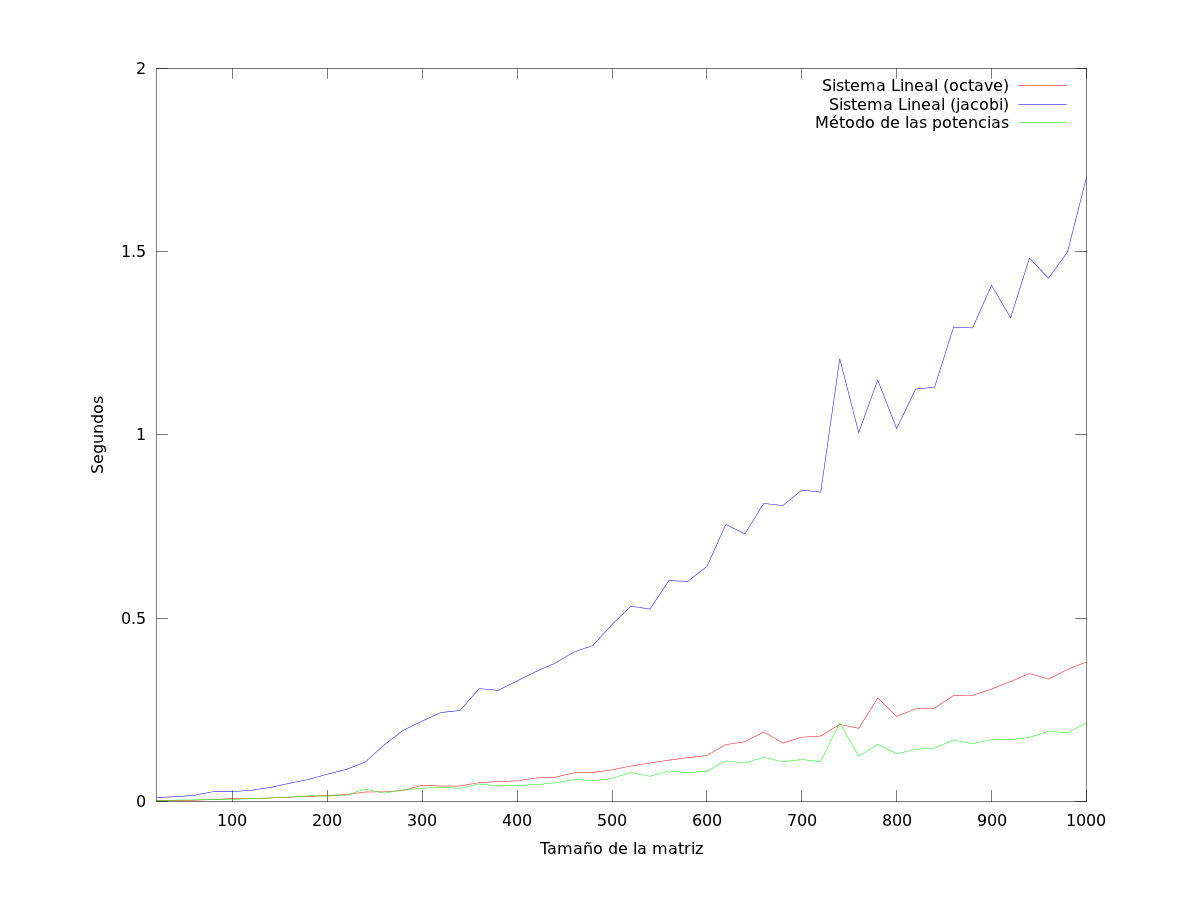
\includegraphics[width=0.5\textwidth]{img/octave_jacobi_pm.png} % [scale=0.75]
    \caption{Gráfico del tiempo de ejecución de los tres algoritmos para grafos web de 20 a 1000 sitios.}
\end{figure}

Es interesante ver (figura 2) que la forma clásica de resolverlo y la resolución por sistema lineal (octave), tienen tiempos bastante similares;
 variando, aparentemente, por tan solo una constante multiplicativa pequeña.
Además, se pueden añadir varias mejoras a ambos algoritmos aún [4] (esta fue una implementacion de los algoritmos básicos), por lo que
 no hay un ganador claro.
Siendo así muy prometedor el nuevo encare por sistemas lineales de ecuaciones, que todavía no está tan explorado.

%----------------------------------------------------------------------
% The bibliography. This bibliography was generated using the following
% two lines:
%\bibliographystyle{IEEEbib}
%\bibliography{ieeecls}
% where, the contents of the ieeecls.bib file was:
%
%@book{lamport,
%        AUTHOR = "Leslie Lamport",
%         TITLE = "A Document Preparation System: {\LaTeX} User's Guide
%                  and Reference Manual",
%       EDITION = "Second",
%     PUBLISHER = "Addison-Wesley",
%       ADDRESS = "Reading, MA",
%          YEAR = 1994,
%          NOTE = "Be sure to get the updated version for \LaTeX2e!"
%}
%
%@book{goossens,
%        AUTHOR = "Michel Goossens and Frank Mittelbach and
%                  Alexander Samarin",
%         TITLE = "The {\LaTeX} Companion",
%     PUBLISHER = "Addison-Wesley",
%       ADDRESS = "Reading, MA",
%          YEAR = 1994,
%}
%
% The ieeecls.bbl file was manually included here to make the distribution
% of this paper easier. You need not do it for your own papers.

\newpage

\section{References}

    [1] Brin, S.; Page, L. (1998). \emph{The anatomy of a large-scale hypertextual Web search engine.}

    [2] Page, L. (1997). \emph{PageRank: Bringing Order to the Web.}

    [3] Bianchini, M.; Gori, M.; Scarselli, F. (2005). \emph{Inside PageRank.}

    [4] Langville, A.; Meyer, C. (2004). \emph{Deeper Inside PageRank.}

    [5] Levering, R.; and M. Cutler. \emph{The Portrait of a Common HTML Web Page}, in DocEng 2006: "Found that the average web page contained 474 words, 281 HTML tags, and 41 links, 10 of which pointed outside the domain"

\end{document}

